% Preamble
\documentclass[a4paper, 12pt, leqno]{article}
\usepackage[margin=1in]{geometry} % Set margin
\usepackage{amssymb,amsmath,amsthm, amsfonts} % Math libraries
\usepackage{pdfpages} % Insert PDF pages

% Hebrew support
\usepackage[utf8x]{inputenc}
\usepackage{culmus}
\usepackage[english,hebrew]{babel}
\selectlanguage{hebrew}

% Custom commands
\newcommand{\sub}[1]{\subsection{\underline{#1}}}
\newcommand{\subsub}[1]{\subsubsection{\underline{#1}}}
\newcommand{\F}{\ensuremath{\mathbb{F}}}
\newcommand{\N}{\ensuremath{\mathbb{N}}}
\newcommand{\Onef}{\ensuremath{1_{\F}}}
\newcommand{\Zerof}{\ensuremath{0_{\F}}}
\newcommand{\eqbcuz}[1]{\text{~$\stackrel{(#1)}{=}$~}}
\newcommand{\eq}[1]{\begin{align*}#1\end{align*}}
\newcommand{\eqn}[1]{\begin{align}#1\end{align}}
\newcommand{\set}[1]{\big{\{} #1 \big{\}}}
\newcommand{\bigset}[1]{\bigg{\{} #1 \bigg{\}}}
\renewcommand{\qed}{\hfill\(\qedsymbol\)}
\renewcommand{\leq}{\leqslant}
\renewcommand{\geq}{\geqslant}
\newcommand{\limn}{\lim_{n\to\infty}}

% Begin Document %
\begin{document}

% Title Page
\begin{titlepage}
    \begin{center}
        \vspace*{4cm}
    
        {\fontsize{32pt}{32pt}\selectfont \textbf{מתמטיקה דיסקרטית 1}}
        
        \vspace{0.4cm}
        
        {\LARGE
        תרגיל 5}
    
        \vfill
            
        {
            \Large\textbf{אביב וקנין}
            \\
            \selectlanguage{english}316017128
        }
    \end{center}
\end{titlepage}

% 1+2
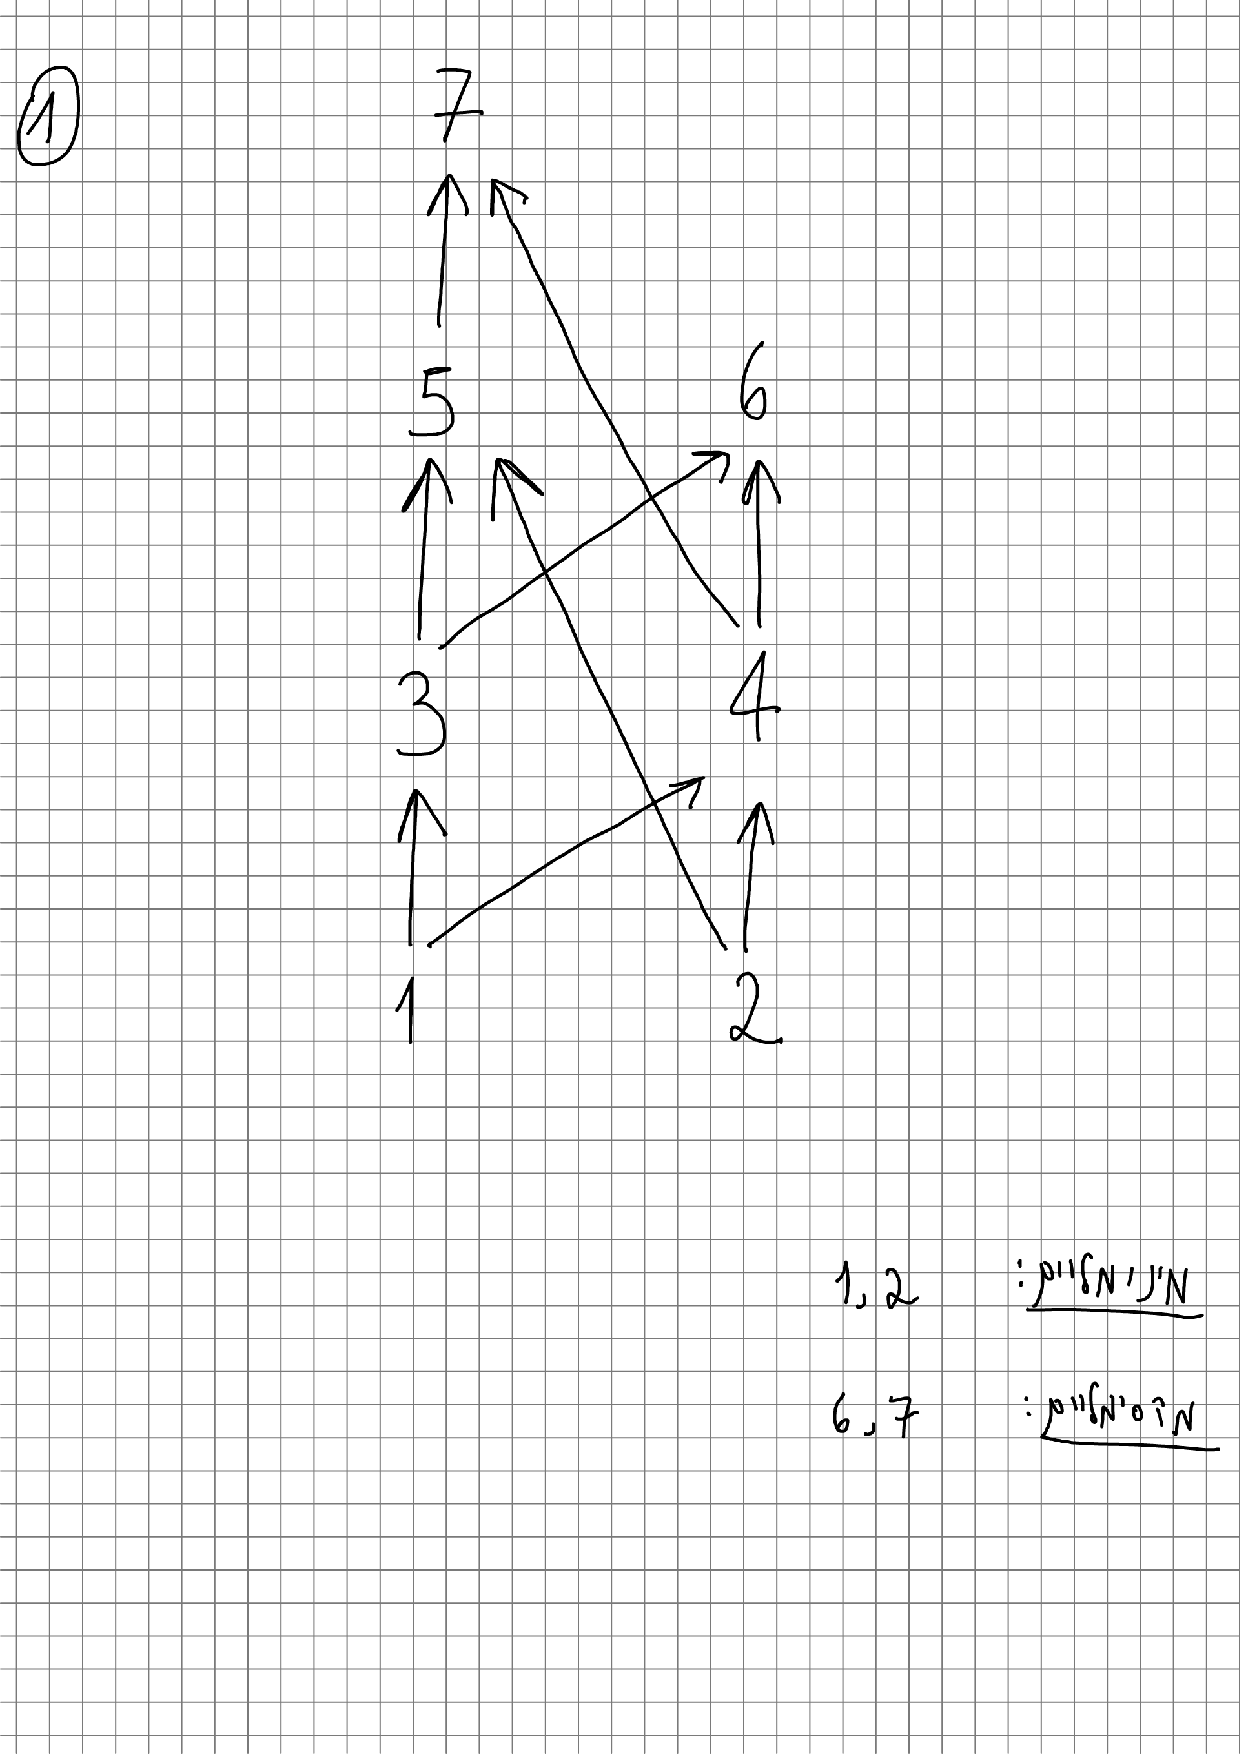
\includepdf[pages=-]{diagrams.pdf}

% 3
\setcounter{section}{2}
\section{}
נניח בשלילה שב-$A$ לא קיים איבר מקסימלי, כלומר:
\eq{
    \forall{a,b}\in{A}~~a\leq{b}
}
הבעיה היא, שיווצר מצב כמו:
\eq{
    a\leq{b}\leq{c}
}
ובמצב זה $c$ הופך להיות האיבר המקסימלי.\\
נוכל להוסיף איבר נוסף $d$, אך נישאר באותו המצב מכיוון שהוא יהיה המקסימלי.\\
סיטואציה זו יכולה להמשיך ללא סוף, אולם נתון כי הקבוצה היא סופית, וזוהי סתירה.
\qed

% 4
\section{כמה מספרים אי־זוגיים בעלי 4 ספרות ניתן להרכיב מהספרות 6, 5, 4, 3, 2, 1 ,כך שבנוסף:}
ראשית, נסמן ב-$A$ את קבוצת המספרים האי-זוגיים בעלי 4 ספרות שניתן להרכיב מ1-6.
\eq{
    |A|=3\cdot6^3
}
\sub{הספרה 1 תופיע לפחות פעם אחת?}
ניקח את $B$ להיות הקבוצה בה הספרה 1 לא מופיעה.
\eq{
    |B|=2\cdot5^3
}
וכעת נחסר את $|B|$ מ-$|A|$ בכדי לקבל את התשובה:
\eq{
    |A|-|B|=3\cdot6^3-2\cdot5^3=398
}
\sub{הספרה 1 תופיע לכל היותר פעם אחת?}
נחלק למקרים.
\subsub{הספרה 1 תופיע פעם אחת בדיוק - $C$}
במידה וספרת האחדות היא 1, יש לנו $5^3$ אפשרויות.
במידה וספרת האחדות אינה 1, יש לנו 3 מקרים שונים של $2\cdot5^2$.
נחבר את המקרים ונקבל:
\eq{
    |C| = 5^3+3(2\cdot5^2) = 275
}
\subsub{הספרה 1 לא תופיע כלל - $D$}
במקרה זה:
\eq{
    |D|=2\cdot5^3=250
}
כעת נחבר את המקרים ונקבל:
\eq{
    |C|+|D|=525
}
\sub{כל הספרות שונות זו מזו?}
במקרה זה יש לנו:
\eq{
    3^2\cdot4\cdot5=180
}

% 5
\section{כמה מספרים בעלי 5 ספרות שונות ניתן להרכיב מ־ 7, 6, 5, 4, 3, 2, 1, 0 כך שהם יתחלקו ב־ 5 וגם יכילו את 5?}
נחלק לשני מקרים:
\sub{ספרת האחדות היא 5 - A}
\eq{
    |A|=4\cdot5\cdot6^2=720
}
\sub{ספרת האחדות היא 0 - B}
\eq{
    |B|=4\cdot(4\cdot5\cdot6)=480
}
נחבר את המקרים ונקבל:
\eq{
    |A|+|B|=1200
}
\pagebreak

% 6
\section{כמה מספרים אי זוגיים בעלי 6 ספרות שונות ניתן להרכיב מהספרות 6, 5, 4, 3, 2, 1 כך שהם יהיו גדולים מהמספר $200000$?}
נחלק לשני מקרים:
\sub{ספרת האחדות היא 1 - A}
\eq{
    |A|=2\cdot3\cdot4\cdot5=120
}
\sub{ספרת האחדות שונה מ-1 - B}
\eq{
    |B|=2^2\cdot3\cdot4^2=192
}
נחבר את המקרים ונקבל:
\eq{
    |A|+|B|=312
}

% 7
\section{בכמה דרכים ניתן להכניס מלפפון, עגבניה, תפוח ואגס למקרר בעל 5 מדפים המסודרים זה מעל זה, כך שהמלפפון יהיה במדף גבוה יותר מהעגבניה? אין הגבלה כלשהי על מספר הפריטים בכל מדף.}
ראשית, נבין כי מכיוון שיש לנו 5 מדפים שונים לדר את התפוח והאגס, אנו מקבלים $25$ אפשרויות שונות:
\eq{
    5^2=25
}
שנית, יש לנו עשר אפשרויות שונות לסידור העגבנייה והמלפפון כך שהמלפפון יהיה מעל העגבנייה, לכן:
\eq{
    10(25)=250
}
לכן, יש $250$ דרכים לעשות זאת.
\pagebreak

% 8
\section{בכמה אופנים ניתן להכניס 6 פירות שונים למקרר בעל 5 מדפים כך שבמדף העליון יהיה בדיוק פרי אחד, במדף
התחתון יהיה בדיוק פרי אחד וגם במדף האמצעי יהיה בדיוק פרי אחד?}
ראשית, נבין כי לאחר סידור 3 הפירות על שלושת המדפים, יישארו לנו 3 פירות ושני מדפים, כלומר:
\eq{
    2^3=8
}
כעת, נחשב את האפשרויות לסידור שלושת המדפים:
\eq{
    6\cdot5\cdot4=120
}
ונקבל את התשובה ע"י כפל מספר האפשרויות:
\eq{
    120\cdot8=960
}

% 9
\section{נתון לוח משבצות בעל 4 עמודות ו־ 6 שורות. בכמה אופנים אפשר לסמן משבצות על הלוח כך שבכל עמודה
תהיה בדיוק משבצת מסומנת אחת, וגם בשורה התחתונה תהיה לכל היותר משבצת מסומנת אחת?}
נחלק למקרים.
\sub{השורה התחתונה מכילה בדיוק משבצת אחת מסומנת - A}
כל עמודה היא מסומנת או לא מסומנת, כלומר יש לנו ארבע אפשרויות.\\
העמודה שהשורה האחרונה שלה מסומנת היא מקרה בעל אפשרות יחידה.
ב-3 העמודות האחרות, יש לנו 5 אפשרויות שונות לסמן כל משבצת נותרת, כלומר:
\eq{
    |A|=4(5^3)=500
}
\sub{השורה התחתונה לא מכילה משבצות מסומנות - B}
כאשר השורה התחתונה אינה משובצת, זה משאיר לנו ארבע עמודות, אשר לכל אחת מהן יש 5 סימונים שונים אפשריים:
\eq{
    |B|=5^4=625
}
נחבר את המקרים ונקבל:
\eq{
    |A|+|B|=500+625=1125
}

% End
\end{document}